\documentclass[11pt]{article}

\usepackage[T1]{fontenc}
\usepackage{lmodern}
\usepackage{microtype}
\usepackage[margin=1in]{geometry}
\usepackage{amsmath,amssymb}
\usepackage{array}
\usepackage{booktabs}
\usepackage{graphicx}
\usepackage{caption}
\usepackage{float}
\usepackage{xurl}
\usepackage{hyperref}

\hypersetup{
  colorlinks=true,
  linkcolor=black,
  citecolor=black,
  urlcolor=blue
}

\title{Computational Notes on Minimal Goldbach Witnesses,\\
Q-free Wall-Spectrum Triage, and Q-line Interval Coverage}
\author{Alex Kulikovsky}
\date{}

\newcommand{\Ne}{N_e}
\newcommand{\lnN}{\log N}
\emergencystretch=2em

\begin{document}
\maketitle

\begin{abstract}
For an even integer \(N\), define the minimal Goldbach witness
\[
  p(N)=\min\{p:\;p\ \text{is prime and}\ N-p\ \text{is prime}\}.
\]
This note reports finite computational experiments around three related
objects: minimal Goldbach witnesses, q-free pre-witness triage for unusually
large witnesses, and fast interval coverage. It is not a proof of the Strong
Goldbach conjecture, not a certified extension of the known verification up to
\(4\cdot10^{18}\), and not a claim that q-line interval coverage is new. The
q-line coverage used here belongs to the classical interval-cover lineage of
Shen and of Deshouillers, te Riele, and Saouter
(Refs.~\ref{ref:shen} and~\ref{ref:deshouillers}).

The present repository contributes a native C/C++ implementation, compact data,
and reproducible finite measurements under explicitly stated primality tests.
The minimal-witness table covers
\[
  \Ne=2\cdot10^e,\qquad e=2,\ldots,5000,
\]
with \(4999\) probable-prime computational witnesses under the GMP primality
test used here. In this table, the largest absolute witness is
\[
  p(2\cdot10^{4718})=549667,
\]
and the largest normalized witness is
\[
  \frac{p(2\cdot10^{3903})}{\log(2\cdot10^{3903})}=58.300567.
\]
A later sparse offset experiment at
\[
  N=2\cdot10^{15000}-77368
\]
found
\[
  p(N)=1{,}223{,}309,\qquad p(N)/\log N=35.417712438.
\]
This row was selected by a q-free scorer and then checked by an increasing
minimal-witness search to \(p_{\max}=2{,}000{,}000\). It is a probable-prime
computational witness under GMP, not a formal primality certificate.

The q-free wall-spectrum benchmark asks whether features computed before the
exact witness search can enrich for large-witness rows. On nine Oliveira e
Silva--Herzog--Pardi least-prime holdout windows, the frozen K3 adaptive policy
covers \(413/450\) benchmark target rows while opening about \(368\) rows per
window, compared with \(346/450\) for a dense wide baseline opening about
\(808\) rows. This is an enrichment result, not a no-skip predictor.

Finally, a separate q-line campaign verifies, under the same probable-prime
convention, \(1.002\cdot10^{12}\) consecutive even values starting at
\(2\cdot10^{19}+2\). The q-lines covered
\(99.999994902\%\) of rows and direct fallback verified the remaining
\(51{,}083\) rows, with no unresolved rows. These are computational witnesses,
not formal primality certificates.

\medskip
\noindent\textbf{Repository:}
\url{https://github.com/alexkulikovskyus/goldbach-computational-lab}
\end{abstract}

\section{Position of This Note}

The even, or Strong, Goldbach conjecture asserts that every even integer
greater than \(2\) is a sum of two primes. This note studies three finite
computational objects related to that conjecture.

The first object is the minimal witness \(p(N)\). It records how far an
increasing search must go before the first decomposition
\[
  N=p+q
\]
is found. This is a stricter measurement than merely finding some
decomposition, because the first successful \(p\) is retained.
Least-prime Goldbach decompositions and related record sequences are known
objects; see, for example, Deshouillers, te Riele, and Saouter
(Ref.~\ref{ref:deshouillers}) and the OEIS entries A025017, A025018, and
A025019 (Ref.~\ref{ref:oeis}).

The second object is q-free wall-spectrum triage. It asks whether features
computed before the exact witness search, and without testing whether
\(q=N-p\) is prime, can enrich for rows with unusually large \(p(N)\).

The third object is interval coverage. It asks for at least one decomposition
for every even \(N\) in a stated finite interval. It does not try to find the
minimal witness for each row. Its purpose is speed: cover many even values at
once, then directly verify any holes.

The distinction matters. A minimal-witness profile is useful for studying
background, spikes, and possible predictors of hard points. Wall-spectrum
triage is a tested way to choose promising neighborhoods before doing exact
witness work. Q-line interval coverage is useful for quickly checking a finite
block, but it does not by itself locate the rows with unusually large
\(p(N)\).

The work reported here should therefore be read as a reproducible computational
study and implementation note. It does not supersede the known complete
verification up to \(4\cdot10^{18}\) by Oliveira e Silva, Herzog, and Pardi,
and it should not be cited as a certified extension of that result
(Ref.~\ref{ref:oliveira}). The q-line campaign begins above that numerical
endpoint, but the evidentiary standard is different: the present rows use GMP
probable-prime tests and have not been upgraded to independent primality
certificates.

\section{Reproducibility Manifest}

The paper is intended to be read together with the public repository. Detailed
file locations, compact result snapshots, public native tools, exact parameter
settings, prior-art guardrails, and current limitations are maintained in the
AI/reviewer context note:
\begin{center}
  \href{https://github.com/alexkulikovskyus/goldbach-computational-lab/blob/main/docs/ai-context-for-paper.md}{\path{docs/ai-context-for-paper.md}}
\end{center}
This keeps the PDF readable while preserving a stable map for reproducing and
auditing the computations.

The GMP workers use \(\texttt{mpz\_probab\_prime\_p}\). GMP returns \(2\) for
a definitely prime value, \(1\) for a probably prime value, and \(0\) for a
composite value (Ref.~\ref{ref:gmpmanual}). In this note, rows accepted by the
workers are therefore called probable-prime computational witnesses unless an
independent certificate is explicitly mentioned.

\section{Residue Classes Modulo 6}

Every prime greater than \(3\) is congruent to either \(1\) or \(5\) modulo
\(6\). This is only a necessary condition, but it is the correct first filter
after removing multiples of \(2\) and \(3\).

For pairs in which both primes are greater than \(3\), the possible residue
lanes are shown in Table~\ref{tab:lanes}.

\begin{table}[H]
\centering
\caption{Allowed prime lanes for \(N=p+q\) modulo \(6\).}
\label{tab:lanes}
\begin{tabular}{cl}
\toprule
\(N \bmod 6\) & possible \((p\bmod 6,\ q\bmod 6)\) \\
\midrule
0 & \((1,5)\) or \((5,1)\) \\
2 & \((1,1)\) \\
4 & \((5,5)\) \\
\bottomrule
\end{tabular}
\end{table}

For the decimal scale-point sequence
\[
  \Ne=2\cdot10^e,
\]
we have \(10^e\equiv4\pmod6\) for all \(e\ge1\), hence
\[
  \Ne\equiv2\pmod6.
\]
Therefore, except for the small exceptional witness \(p=3\), every successful
pair on this sequence must satisfy
\[
  p\equiv1\pmod6,\qquad q\equiv1\pmod6.
\]
The completed scale-point data match this exactly: among \(4999\) rows,
\(4984\) witnesses are \(1\bmod6\), \(15\) are the exceptional value \(3\),
and none are \(5\bmod6\).

\begin{figure}[!htbp]
\centering
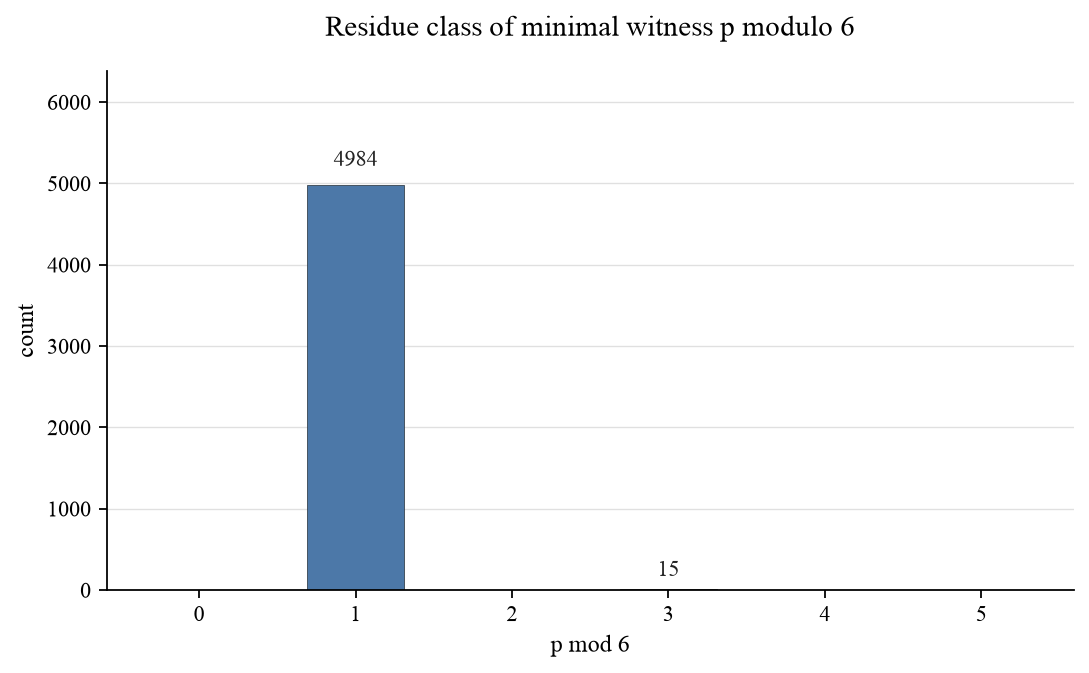
\includegraphics[width=0.62\linewidth]{figures/scale-point-p-mod6.png}
\caption{Residue class of \(p(N_e)\) modulo \(6\). Non-exceptional witnesses lie in the \(1\bmod6\) lane.}
\label{fig:mod6}
\end{figure}

\section{Minimal-Witness Computation}

For a fixed even integer \(N\), the minimal-witness workers test prime
candidates \(p\) in increasing numerical order. For each candidate they form
\[
  q=N-p.
\]
The first accepted candidate is recorded as \(p(N)\). Thus the word
\emph{minimal} always refers to the ordering of \(p\), not to the size of
\(q\), and not to a later choice among many possible decompositions.

The search uses three filters.
\begin{enumerate}
\item Candidate \(p\) must be prime and below the configured bound
  \(p_{\max}\).
\item The pair \((p,q)\) must lie in an admissible modulo-\(6\) lane. This
  removes only candidates for which \(q\) is forced to be divisible by \(2\)
  or \(3\), except for explicit small-prime cases.
\item The remaining \(q\) is tested for primality. In the GMP workers this is
  \texttt{mpz\_probab\_prime\_p} with \(25\) repetitions for accepted rows.
\end{enumerate}

The public scale-point table uses
\[
  N_e=2\cdot10^e,\qquad e=2,\ldots,5000,
\]
with \(p_{\max}=1{,}000{,}000\). Every reported row found a witness below this
bound. The resulting rows are probable-prime computational witnesses under
the primality test used by the worker.

The contiguous C verifier scans every even \(N\) in a finite interval. It uses
pthread workers, a segmented bitset sieve for odd \(q\), base primes up to the
square root of the interval endpoint, and a \(2\cdot3\cdot5\cdot7=210\) wheel
prefilter. For \(N\equiv0\pmod6\), both admissible lanes are merged in
increasing \(p\) order, so the recorded value is the global first witness.

\begin{table}[!htbp]
\centering
\caption{Main parameters used in the minimal-witness runs.}
\label{tab:parameters}
\begin{tabular}{lll}
\toprule
Computation & parameter & value \\
\midrule
Contiguous range runs & CPU workers & 18 \\
Contiguous range runs & segment width & \(5{,}000{,}000\) \\
Contiguous range runs & \(p_{\max}\) & \(100{,}000\) \\
Scale-point run & exponents & \(2,\ldots,5000\) \\
Scale-point run & \(p_{\max}\) & \(1{,}000{,}000\) \\
Scale-point run & GMP repetitions & 25 \\
Survivor-pressure scan & exponents & \(201,\ldots,5000\) \\
Survivor-pressure scan & \(\texttt{smallLimit}\) & \(250{,}000\) \\
Survivor-pressure scan & \(\texttt{factorLimit}\) & \(250{,}000\) \\
\bottomrule
\end{tabular}
\end{table}

\section{Contiguous Range Results}

Table~\ref{tab:range} summarizes two local finite-interval minimal-witness
runs. Both used 18 CPU workers, segment width \(5{,}000{,}000\), and candidate
limit \(p\le100{,}000\).

\begin{table}[!htbp]
\centering
\caption{Contiguous finite-interval minimal-witness runs.}
\label{tab:range}
\begin{tabular}{lrrrrrrr}
\toprule
Range & even values & time & failures & mean attempts & median & q99 & max \(p\) \\
\midrule
\(20\mathrm{B}\ldots100\mathrm{B}\) & \(40{,}000{,}000{,}001\) & \(54.638\)s & 0 & \(8.336624\) & 6 & 35 & 2803 \\
\(100\mathrm{B}\ldots1\mathrm{T}\) & \(450{,}000{,}000{,}001\) & \(718.832\)s & 0 & \(9.056742\) & 7 & 39 & 3457 \\
\bottomrule
\end{tabular}
\end{table}

The maximum-witness cases in these two runs were
\[
  35{,}884{,}080{,}836 = 2803 + 35{,}884{,}078{,}033
\]
and
\[
  599{,}533{,}546{,}358 = 3457 + 599{,}533{,}542{,}901.
\]
These runs are modest in mathematical scope, but useful as local performance
and background measurements.

\section{\texorpdfstring{Scale Points Through \(e=5000\)}{Scale Points Through e=5000}}

The decimal scale-point table contains \(4999\) rows:
\[
  N_e=2\cdot10^e,\qquad e=2,\ldots,5000.
\]
The repository includes a compact table containing the exponent, witness
\(p\), residue class, normalized ratio, attempt counts, and verification flag.
The enormous \(q=N_e-p\) values are omitted from the public table to keep the
repository compact. Summary statistics are shown in Table~\ref{tab:summary}.

\begin{table}[!htbp]
\centering
\caption{Summary of the full scale-point table.}
\label{tab:summary}
\begin{tabular}{lr}
\toprule
Statistic & value \\
\midrule
completed scale points & 4999 \\
median \(p(N)\) & 14407 \\
mean \(p(N)\) & 31973.490098 \\
90th percentile \(p(N)\) & 84223 \\
95th percentile \(p(N)\) & 121789 \\
99th percentile \(p(N)\) & 225157 \\
maximum \(p(N)\) & 549667 at \(e=4718\) \\
median \(p(N)/\log N\) & 3.277880 \\
mean \(p(N)/\log N\) & 5.289201 \\
99th percentile \(p(N)/\log N\) & 27.782478 \\
maximum \(p(N)/\log N\) & 58.300567 at \(e=3903\) \\
\bottomrule
\end{tabular}
\end{table}

The bucketed behavior by exponent range is shown in Table~\ref{tab:buckets}.
The absolute witness tends to grow with scale, but unevenly. The normalized
quantity \(p(N)/\log N\) remains noisy and spike-driven rather than monotone.

\begin{table}[!htbp]
\centering
\caption{Scale-point buckets by exponent.}
\label{tab:buckets}
\begin{tabular}{rrrrrr}
\toprule
\(e\)-range & points & median \(p\) & p99 \(p\) & max \(p\) & median \(p/\log N\) \\
\midrule
2--1000 & 999 & 2659 & 38977 & 64879 & 2.939861 \\
1001--2000 & 1000 & 11053 & 93529 & 139831 & 3.151170 \\
2001--3000 & 1000 & 19282 & 158941 & 280927 & 3.349864 \\
3001--4000 & 1000 & 26482 & 237073 & 523987 & 3.275531 \\
4001--5000 & 1000 & 37141 & 301867 & 549667 & 3.650981 \\
\bottomrule
\end{tabular}
\end{table}

The large-scale absolute records after \(e=1000\) occur at
\[
\begin{gathered}
1310,\,2040,\,2079,\,2744,\,3273,\,3414,\,3794,\,3903,\,4718,\\
p(N_e)=139831,\,187597,\,276037,\,280927,\,302299,\,327559,\,348571,\,523987,\,549667.
\end{gathered}
\]

\begin{figure}[!t]
\centering
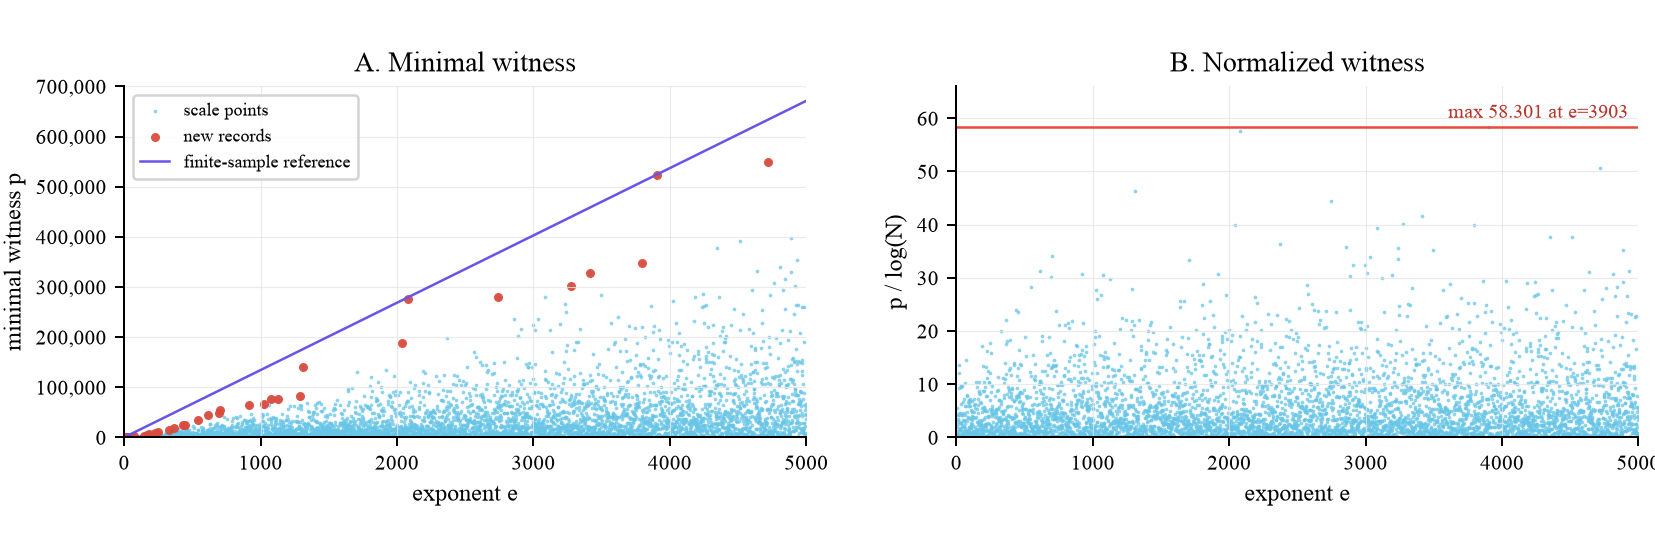
\includegraphics[width=0.95\linewidth]{figures/scale-point-two-panel.png}
\caption{Scale-point minimal witnesses and normalized witness ratios for \(N_e=2\cdot10^e\), \(e=2,\ldots,5000\). Red points in panel A mark new absolute records; the blue line is a finite-sample reference, not a bound.}
\label{fig:minp}
\label{fig:ratio}
\end{figure}

\section{\texorpdfstring{A Targeted Sparse-Scale Experiment at \(e=15000\)}{A Targeted Sparse-Scale Experiment at e=15000}}

The scale-point grid \(N_e=2\cdot10^e\) is intentionally simple, but it is
also sparse in a restrictive way: it samples only one even integer per
exponent. After the \(e\le5000\) table and the later \(e=10000\) offset tests,
we ran a more targeted experiment around
\[
  N=2\cdot10^{15000}+\Delta
\]
with small even offsets \(\Delta\). The motivation was not that larger \(e\)
should automatically produce a larger witness. Rather, the normalization
changes the threshold. At \(e=10000\), \(p=10^6\) corresponds to
\[
  p/\log N \approx 43.428140873,
\]
whereas at \(e=15000\) it corresponds to
\[
  p/\log N \approx 28.952384424.
\]
The previous offset record at \(e=10000\),
\[
  p(2\cdot10^{10000}-38602)=634091,
\]
had \(p/\log N\approx27.537393274\). Thus a million-sized witness at
\(e=15000\) required only a modest normalized improvement over that local
record.

The experiment used a three-stage procedure.
\begin{enumerate}
\item A q-free pressure scout scanned offsets
  \[
    -100000\le\Delta\le100000,\qquad \Delta\equiv0\pmod2,
  \]
  with \(\texttt{pLimit}=10000\), small-factor depths \(97\) and \(997\), and
  retained the top \(200\) offsets.
\item The retained offsets were converted into full GMP input rows and scored
  by the q-free survivor-road scorer to \(p_{\max}=1{,}000{,}000\), using
  \(\texttt{smallLimit}=250000\). This scorer does not test \(q=N-p\) for
  primality. It records only the admissible modulo-\(6\) lane, the
  small-prime blockers of \(q\), survivor density, milestone positions such
  as \(p\) at the 1000th survivor, and bucketed road geometry.
\item The exact basket was frozen before witness computation. It mixed the
  strongest \(N\bmod6=4\) road-bucket rows with the strongest \(N\bmod6=2\)
  rank-sum rows from the scorer output. This was a selection rule for a small
  experiment, not a proof that all high-witness offsets must pass through the
  same bucket.
\item A small exact basket of ten offsets was then checked by the
  increasing minimal-witness worker with \(18\) threads and GMP
  \(\texttt{primalityReps}=5\).
\end{enumerate}

Table~\ref{tab:e15000top10} gives the exact results for that basket. One row,
\(\Delta=-77368\), had no witness below \(10^6\). A deeper single-row run to
\(p_{\max}=2{,}000{,}000\) found the first witness at \(p=1{,}223{,}309\).

\begin{table}[!htbp]
\centering
\caption{Targeted \(e=15000\) offset basket. Rows are probable-prime computational witnesses under the GMP test used here.}
\label{tab:e15000top10}
\small
\begin{tabular}{rrrrrr}
\toprule
offset \(\Delta\) & \(10^6\) pass & final \(p(N)\) & \(p/\log N\) & pass s & deep s \\
\midrule
\(-77368\) & no witness & \(1{,}223{,}309\) & \(35.417712438\) & \(1845.52\) & \(2257.19\) \\
\(64214\) & \(432{,}737\) & \(432{,}737\) & \(12.528767979\) & \(883.538\) & -- \\
\(69758\) & \(386{,}537\) & \(386{,}537\) & \(11.191167818\) & \(823.556\) & -- \\
\(64268\) & \(381{,}047\) & \(381{,}047\) & \(11.032219228\) & \(915.606\) & -- \\
\(41828\) & \(358{,}607\) & \(358{,}607\) & \(10.382527721\) & \(743.347\) & -- \\
\(46362\) & \(299{,}191\) & \(299{,}191\) & \(8.662292848\) & \(695.728\) & -- \\
\(89862\) & \(190{,}369\) & \(190{,}369\) & \(5.511636471\) & \(441.525\) & -- \\
\(9138\) & \(127{,}837\) & \(127{,}837\) & \(3.701185968\) & \(295.304\) & -- \\
\(-10134\) & \(90{,}373\) & \(90{,}373\) & \(2.616513838\) & \(234.865\) & -- \\
\(-93048\) & \(7{,}459\) & \(7{,}459\) & \(0.215955835\) & \(38.746\) & -- \\
\bottomrule
\end{tabular}
\end{table}

\begin{figure}[H]
\centering
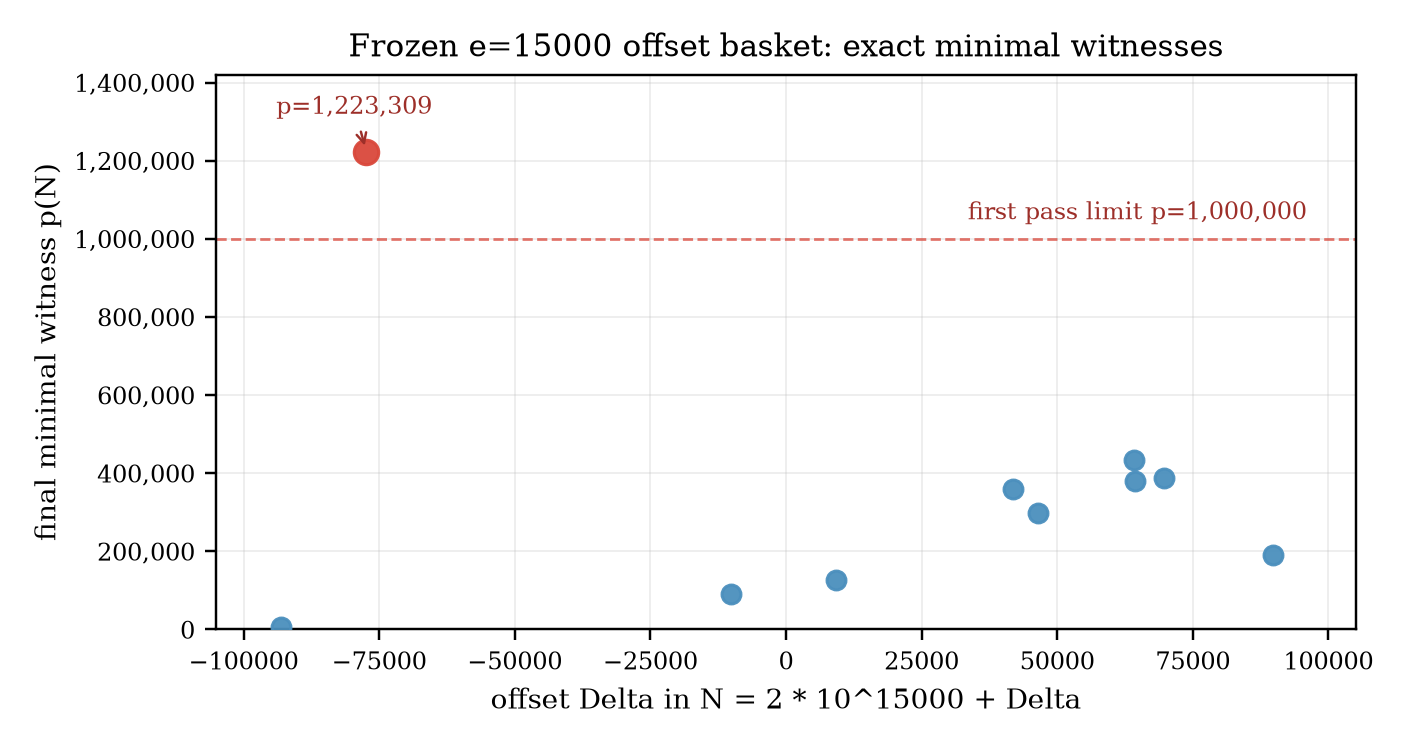
\includegraphics[width=0.54\linewidth]{figures/e15000-offset-basket.png}
\caption{Exact results for the frozen \(e=15000\) offset basket. The highlighted row is the offset that had no witness below \(10^6\) and was then resolved at \(p(N)=1{,}223{,}309\).}
\label{fig:e15000basket}
\end{figure}

The result is encouraging but should be stated carefully. The least-prime
Goldbach partition \(p(N)\) is a standard object in the literature and in the
Oliveira e Silva--Herzog--Pardi data (Ref.~\ref{ref:oliveira}). The present
experiment does not introduce that object, does not verify a consecutive
range, and does not prove a predictor. Its narrower contribution is a
reproducible sparse-scale measurement: a q-free road-scoring pass selected a
small basket that contained a row with \(p(N)>10^6\), and the exact worker
then located the witness \(p(N)=1{,}223{,}309\).

The negative information is also useful. Several highly ranked rows produced
ordinary witnesses, and the \(N\bmod6=2\) rank-sum candidates were noisier
than the \(N\bmod6=4\) road bucket in this run. The current scorer is
therefore an enrichment device, not a no-skip rule.

\section{Survivor Pressure}

The first witness \(p(N)\) records where the increasing search stops. To study
why the search lasted that long, we also record the failures before the first
success. After the modulo-\(6\) lane and the small-prime wall have removed the
obvious composites, some candidates remain for which
\[
  q=N-p
\]
is not divisible by the small primes but is still composite. We call the
number of such failed candidates before the first witness the survivor
pressure of \(N\), for the chosen small-prime bound.

More formally, fix a small-prime bound \(L\). For an admissible prime
candidate \(p<p(N)\), define the small-prime wall to block \(p\) if there is a
prime \(r\), \(5\le r\le L\), such that
\[
  r\mid(N-p).
\]
The survivor pressure is then
\[
  \begin{aligned}
  S_L(N)=\#\{p<p(N):\;&p\ \text{prime},\ p\ \text{admissible},\\
  &N-p\ \text{passes the small-prime wall but is composite}\}.
  \end{aligned}
\]
In this note survivor pressure is a post-hoc diagnostic and ranking statistic.
It is not an independent formula for predicting \(p(N)\), because it is
measured only up to an already known first witness.

\begin{table}[!htbp]
\centering
\caption{Top scale points by survivor pressure, \(201\le e\le5000\).}
\label{tab:pressure}
\begin{tabular}{rrrrrr}
\toprule
\(e\) & \(p(N_e)\) & \(p/\log N\) & pressure & small-wall blocks & admissible \\
\midrule
4718 & 549667 & 50.593920 & 3591 & 19032 & 22624 \\
3903 & 523987 & 58.300567 & 3397 & 18268 & 21666 \\
4887 & 397519 & 35.324263 & 2648 & 14143 & 16792 \\
4514 & 391873 & 37.699808 & 2602 & 13964 & 16567 \\
4349 & 378253 & 37.770021 & 2544 & 13505 & 16050 \\
4929 & 354169 & 31.203946 & 2374 & 12749 & 15124 \\
3794 & 348571 & 39.897325 & 2358 & 12542 & 14901 \\
4641 & 331663 & 31.034275 & 2293 & 11957 & 14251 \\
4811 & 340381 & 30.724660 & 2290 & 12287 & 14578 \\
4885 & 329617 & 29.302359 & 2267 & 11901 & 14169 \\
\bottomrule
\end{tabular}
\end{table}

Across the \(4800\) scale-point rows \(e=201,\ldots,5000\), the Pearson
correlation between \(p(N_e)\) and survivor pressure is \(0.997643\). This high
value is expected because pressure is measured up to the already-known first
witness. The correlation between \(p(N_e)/\log N_e\) and survivor pressure is
lower, \(0.851063\), because the normalized quantity also depends on the size
of \(N_e\).

The empirical use of survivor pressure is therefore modest but real. It
describes the path that the minimal-witness search had to take, and it gives a
way to rank already computed scale points for local follow-up.

\section{Q-free Wall-Spectrum Triage}

Survivor pressure is post-hoc because it is measured only up to a known first
witness. A more useful question is whether a related signal can be computed
before the exact witness search. The wall-spectrum experiments test this
question.

For an even \(N\), and for early admissible prime candidates \(p\), define a
candidate to be blocked at wall depth \(L\) if \(N-p\) has a prime divisor
at most \(L\). This uses only divisibility by small primes. It does not test
whether \(N-p\) is prime and it does not use the exact value of \(p(N)\).
Across a local window, the resulting small-divisor pressure forms a
wall-spectrum: a sequence of local pressure highs and lows across several
wall depths.

The current best frozen policy is called K3 adaptive wall persistence. In
plain terms, it:
\begin{enumerate}
\item scores several wall-depth layers;
\item finds local q-free pressure maxima in each layer;
\item keeps centers that persist across layers;
\item opens small adaptive neighborhoods around the strongest centers;
\item uses exact minimal-witness labels only afterward, for evaluation.
\end{enumerate}

For reproducibility, Table~\ref{tab:k3params} lists the frozen K3 parameters
used in the frontier below. The feature layers use equal \(p\)-candidate and
wall limits at each depth.

\begin{table}[!htbp]
\centering
\caption{Frozen K3 adaptive wall-persistence parameters.}
\label{tab:k3params}
\begin{tabular}{ll}
\toprule
Parameter & value \\
\midrule
feature layers & \(5000,8000,9000,10000,12000\) \\
window radius & \(\pm2000\) rows \\
labels & minimal-witness labels used only for evaluation \\
label limits & \(\texttt{pLimit}=50000,\ \texttt{smallLimit}=50000\) \\
layer local suppression & \(\texttt{layerSuppress}=20\) \\
layer centers & \(\texttt{layerTopK}=3\) \\
persistence vote radius & \(\texttt{voteR}=20\) \\
final center suppression & \(\texttt{finalSuppress}=100\) \\
final centers & \(\texttt{finalTopK}=10\) \\
base reveal radius & \(\texttt{baseR}=20\) \\
adaptive expansion & \(\texttt{expandTop}=4,\ \texttt{expandR}=60\) \\
\bottomrule
\end{tabular}
\end{table}

The benchmark uses known large-witness rows from the Oliveira
e Silva--Herzog--Pardi least-prime data (Ref.~\ref{ref:oliveira}). One
benchmark group consists of a known least-prime row and the contiguous
\(\pm2000\)-row local window around it. The feature stage receives the even
values in that local window, computes only q-free small-divisor features, and
opens a subset of rows. A hit means that the opened subset contains the known
least-prime row. Exact minimal witnesses are used only afterward as labels for
evaluation; they are not available to the feature stage.

Table~\ref{tab:wallfrontier} gives the current comparable frontier. The nine
fresh holdout blocks cover least-prime ranks \(51\)--\(500\), grouped into
fifty-row windows. Each policy in the table is measured on the same \(450\)
benchmark groups. The ``dense'' baselines use single-layer dense local maxima
with fixed or adaptive reveal radii; K3 uses persistence across the five
feature layers in Table~\ref{tab:k3params}.

\begin{table}[!htbp]
\centering
\caption{Q-free wall-spectrum holdout frontier on least-prime local windows.}
\label{tab:wallfrontier}
\begin{tabular}{lrrrr}
\toprule
Policy & holdouts & hits & hit rate & mean opened rows \\
\midrule
K3 adaptive & 9 & \(413/450\) & \(91.78\%\) & 368.30 \\
dense wide & 9 & \(346/450\) & \(76.89\%\) & 807.96 \\
dense adaptive & 9 & \(298/450\) & \(66.22\%\) & 347.36 \\
dense strict & 9 & \(287/450\) & \(63.78\%\) & 206.89 \\
\bottomrule
\end{tabular}
\end{table}

The positive result is that K3 adaptive covers substantially more target rows
than dense wide while opening less than half as many rows. The negative result
is equally important: K3 adaptive still misses \(37/450\) target rows. The
tested rule is therefore a triage and enrichment method, not a formula and not
a no-skip localizer.

Two variants were also checked because earlier inspected blocks made them look
promising. The fresh candidate-validation block was least-prime ranks
\(451\)--\(500\). It did not promote either variant over K3, as shown in
Table~\ref{tab:wallcandidates}.

\begin{table}[!htbp]
\centering
\caption{Fresh candidate validation on least-prime ranks \(451\)--\(500\).}
\label{tab:wallcandidates}
\begin{tabular}{lrrl}
\toprule
Policy & hits & mean opened rows & interpretation \\
\midrule
K3 adaptive & \(48/50\) & 368.32 & current baseline \\
MassR100 priority & \(47/50\) & 365.20 & cheaper, but loses one hit \\
confidence tier & \(48/50\) & 442.04 & ties K3, but costs more \\
\bottomrule
\end{tabular}
\end{table}

The two K3 misses in the fresh candidate-validation block are informative.
In both cases the true target was near a selected wall center, but the opened
radius was too small. This supports the same interpretation: the wall-spectrum
signal often lands near hard rows, but the tested reveal geometry is not safe
enough to discard all unopened rows.

\section{Q-line Interval Coverage}

The q-line calculation is a different computation. It does not compute
\(p(N)\). It tries to prove a weaker finite statement: for every even \(N\) in
a stated finite block, find at least one decomposition \(N=p+q\) under the
primality tests used by the worker.

The idea is classical. Shen used a digital computer to check Goldbach up to
\(33{,}000{,}000\) (Ref.~\ref{ref:shen}), and Sinisalo later checked up to
\(4\cdot10^{11}\) (Ref.~\ref{ref:sinisalo}). Granville, te Riele, and van de
Lune studied checking Goldbach on a vector computer
(Ref.~\ref{ref:granville}).
Deshouillers, te Riele, and Saouter later described interval algorithms in
terms of finding sets of primes \(P\) and \(Q\) such that \(P+Q\) covers all
even values in an interval (Ref.~\ref{ref:deshouillers}). Their Cray
implementation used bit arrays and shifted copies of prime arrays. The present
q-line worker uses the same general reversal: choose many prime \(q\)'s near
the interval, then use a prime bitset for the smaller moving part \(p\).

For one block, let \(N_0\) be a chosen anchor near the block. For an odd value
\(a\), define
\[
  q_a=N_0-a.
\]
If \(q_a\) is prime, then for each even \(N\) in the block the corresponding
candidate is
\[
  p_a(N)=N-q_a=a+(N-N_0).
\]
The q-line covers exactly the rows for which \(p_a(N)\) is also prime. One
prime \(q_a\) can therefore cover many rows.

The worker builds many such lines. Candidate \(q_a\)'s are first filtered by
small primes up to \(\texttt{qFilterLimit}\), then tested with GMP. The moving
\(p\)-side is represented by an ordinary prime bitset over the needed
integer range. The block coverage bitset is updated by OR-ing the shifted
prime slices from all accepted q-lines.

Rows not covered by q-lines are not discarded. Each uncovered row is sent to a
direct fallback search. A finite block is accepted only when
\[
  \texttt{qlineRows}+\texttt{fallbackVerified}=\texttt{rows},
  \qquad
  \texttt{unresolved}=0.
\]
This no-skip condition is the important safety rule. A q-line miss is only a
miss by the current q-line geometry; it is not evidence against Goldbach and
not automatically a minimal-witness peak.

\section{\texorpdfstring{The \(e19\)-forward Q-line Campaign}{The e19-forward Q-line Campaign}}

The completed q-line campaign reported here starts at
\[
  B=2\cdot10^{19}
\]
and scans consecutive even values
\[
  N=B+\texttt{offset}.
\]
The offsets range from \(2\) to \(2{,}004{,}000{,}000{,}000\). Equivalently,
the checked even interval is
\[
  2\cdot10^{19}+2
  \le N \le
  2\cdot10^{19}+2{,}004{,}000{,}000{,}000.
\]
The interval contains \(1{,}002{,}000{,}000{,}000\) even values, split into
\(1002\) blocks of \(1{,}000{,}000{,}000\) rows.

The campaign parameters are shown in Table~\ref{tab:qlineparams}.

\begin{table}[!htbp]
\centering
\caption{Parameters for the \(e19\)-forward q-line campaign.}
\label{tab:qlineparams}
\begin{tabular}{lr}
\toprule
Parameter & value \\
\midrule
rows per block & \(1{,}000{,}000{,}000\) \\
blocks & \(1002\) \\
\(\texttt{aLimit}\) & \(50{,}000\) \\
\(\texttt{pLimit}\) for direct fallback & \(250{,}000\) \\
\(\texttt{qFilterLimit}\) & \(250{,}000\) \\
\(\texttt{smallLimit}\) for fallback & \(250{,}000\) \\
GMP repetitions & 25 \\
block-parallel jobs & 18 \\
\bottomrule
\end{tabular}
\end{table}

The aggregate result is shown in Table~\ref{tab:qlinecampaign}.

\begin{table}[!htbp]
\centering
\caption{Aggregate result of the \(e19\)-forward q-line campaign.}
\label{tab:qlinecampaign}
\begin{tabular}{lr}
\toprule
Quantity & value \\
\midrule
even values checked & \(1{,}002{,}000{,}000{,}000\) \\
rows covered by q-lines & \(1{,}001{,}999{,}948{,}917\) \\
q-line coverage share & \(99.999994902\%\) \\
direct fallback rows & \(51{,}083\) \\
direct fallback rows verified & \(51{,}083\) \\
unresolved rows & 0 \\
accepted q-lines, summed by block & \(1{,}127{,}333\) \\
GMP tests for q-line candidates & \(3{,}388{,}627\) \\
GMP tests in direct fallback & \(167{,}760\) \\
total q-side GMP tests & \(3{,}556{,}387\) \\
average fallback rows per billion & \(50.981038\) \\
minimum fallback rows in a block & 4 \\
maximum fallback rows in a block & 207 \\
\bottomrule
\end{tabular}
\end{table}

The result should be phrased narrowly:
\[
\begin{gathered}
\text{Every tested even }N\text{ in this finite interval had at least one}\\
\text{Goldbach decomposition under the GMP probable-prime tests used here.}
\end{gathered}
\]
This is not a statement about untested integers. It is not a minimal-witness
profile over the interval. It is also not a formal certificate unless the
accepted large primes are later independently certified.

\section{Contribution and Limits}

The q-line idea itself is not new; the relevant prior art is explicitly cited
above and in the references. The appropriate claim is more limited: the
repository provides a compact modern implementation, a reproducible data
snapshot, and engineering measurements for a large interval above \(2\cdot
10^{19}\) under a clearly stated probable-prime convention.

The same caution applies to minimal Goldbach witnesses. The least-prime
partition \(p(N)\), first-occurrence tables \(S(p)\), and record-holders for
minimal Goldbach partitions are prior work, not inventions of this project.
The Oliveira e Silva project page explicitly defines the minimal Goldbach
partition and reports top least-prime record data below \(4\cdot10^{18}\)
(Ref.~\ref{ref:oliveira}). The targeted \(e=15000\) result in this note is
different in scope: it is a sparse, very large decimal-scale point, selected
by q-free triage and checked under GMP probable-prime tests. It should be read
as an experimental measurement and a test of the triage workflow.

The most useful observations are practical. Minimal-witness data,
wall-spectrum triage, and q-line coverage answer different questions. The
first measures \(p(N)\). The second tries to choose promising neighborhoods
before the exact witness search. The third finds any valid decomposition in a
finite block. On the scale-point grid \(2\cdot10^e\), \(p(N_e)\) behaves like a
noisy spike process rather than a monotone formula. Survivor pressure is a
diagnostic of an already computed row, not a proven predictor. The
wall-spectrum benchmark shows a reproducible q-free enrichment signal: K3
adaptive covers more known benchmark target rows than dense wide at lower
opened-row cost. It also shows the boundary of the present method: the rule
still misses target rows, and the first fresh MassR100/tier candidate validation did not
improve the K3 frontier.

In the q-line campaign, almost all rows were covered by shifted prime bitsets,
and the tiny residue was handled by direct fallback. The fallback layer is the
implementation detail that keeps the method no-skip for interval coverage. The
resulting finite coverage is reproducible, but the present standard is
probable-prime computation; independent primality certificates have not yet
been produced for these rows.

In the sparse offset campaign, the q-free survivor-road scorer found a basket
containing
\[
  N=2\cdot10^{15000}-77368,\qquad p(N)=1{,}223{,}309.
\]
This is the strongest single minimal-witness row currently reported by this
project. The restrained conclusion is that the road-score triage can enrich a
small exact basket for unusually delayed witnesses. The equally important
limitation is that the same basket contained several ordinary rows; the
method is not a formula for locating all large witnesses.

The present data therefore justify an open repository and a computational note.
They do not justify claiming a new proof of Goldbach, a no-skip formula for
minimal witnesses, a new discovery of q-line coverage, or a certified extension
of the known complete verification.

\section*{Acknowledgements}

The project is indebted to earlier work by Shen; Sinisalo; Granville, te Riele,
and van de Lune; Deshouillers, te Riele, and Saouter; Richstein; and Oliveira
e Silva, Herzog, and Pardi. Drafting, code-review, and computational workflow
assistance were provided by Codex.

\section*{References}

\small
\begin{enumerate}
\setlength{\itemsep}{0pt}
\setlength{\parskip}{0pt}
\item\label{ref:shen} M.-K. Shen, ``On checking the Goldbach conjecture,'' \emph{BIT
Numerical Mathematics}, 4, 243--245, 1964.
\item\label{ref:sinisalo} M. K. Sinisalo, ``Checking the Goldbach conjecture up to
\(4\cdot10^{11}\),'' \emph{Mathematics of Computation}, 61(204), 931--934,
1993.
\item\label{ref:granville} A. Granville, H. J. J. te Riele, and J. van de Lune,
``Checking the Goldbach conjecture on a vector computer,'' in
\emph{Number Theory and Applications}, R. A. Mollin, ed., Kluwer Academic
Publishers, 423--433, 1989.
\item\label{ref:deshouillers} J.-M. Deshouillers, H. J. J. te Riele, and Y. Saouter, ``New
experimental results concerning the Goldbach conjecture,'' \emph{ANTS-III},
LNCS 1423, 204--215, 1998.
\item\label{ref:richstein} J. Richstein, ``Verifying the Goldbach conjecture up to
\(4\cdot10^{14}\),'' \emph{Mathematics of Computation}, 70(236),
1745--1749, 2001.
\item\label{ref:oliveira} T. Oliveira e Silva, S. Herzog, and S. Pardi, ``Empirical verification
of the even Goldbach conjecture and computation of prime gaps up to
\(4\cdot10^{18}\),'' \emph{Mathematics of Computation}, 83(288), 2033--2060,
2014. \url{https://sweet.ua.pt/tos/goldbach.html}.
\item\label{ref:oeis} OEIS Foundation Inc., entries A025017, A025018, and
A025019, least-prime Goldbach partition sequences.
\url{https://oeis.org/A025017}, \url{https://oeis.org/A025018},
\url{https://oeis.org/A025019}.
\item\label{ref:gmp} GNU MP: The GNU Multiple Precision Arithmetic Library.
\url{https://gmplib.org/}.
\item\label{ref:gmpmanual} GNU MP Manual, ``Number Theoretic Functions,''
documentation for \(\texttt{mpz\_probab\_prime\_p}\).
\url{https://gmplib.org/manual/Number-Theoretic-Functions.html}.
\end{enumerate}

\end{document}
